% !TeX root = main.tex

\documentclass[11pt]{article}

\usepackage[utf8]{inputenc}
\usepackage{amsmath, amssymb}
\usepackage{geometry}
\usepackage{graphicx}
\usepackage{tikz}
\usepackage{hyperref}
\usepackage{enumitem}
\usepackage{titlesec}
\usepackage{float}
\usepackage{tikz}               
\usetikzlibrary{arrows.meta, positioning}

\geometry{margin=1in}
\titleformat{\section}[block]{\large\bfseries}{\thesection}{1em}{}
\titleformat{\subsection}[block]{\normalsize\bfseries}{\thesubsection}{1em}{}

% === Metadata ===
\title{LLM Benchmarking Framework for Description Logic Reasoning}
\author{Phanphum Prathumsuwan\\Mahidol University\\phanphum.pra@student.mahidol.ac.th}
\date{\today}

\begin{document}

\maketitle

% --- Abstract ---
\begin{abstract}
This paper presents a novel benchmarking framework to evaluate the Description Logic (DL) reasoning capabilities of Large Language Models (LLMs). 
While prior work has tested LLMs on symbolic reasoning and natural language inference\cite{leapofthought2020,han2022folio}, few have focused on the structured semantics of DL, particularly the EL and ELH fragments widely used in ontology engineering\cite{baader2005el}. 
The framework extracts EL axioms from the Pizza ontology\cite{stanford2025pizza, horridge2004pizza} and extends them with role inclusion to create ELH-compliant cases, thereby increasing DL complexity. It then generates corresponding natural language queries, and compares model responses to formal entailment outcomes using the OWL API\cite{owlapi} and HermiT reasoner\cite{hermit2007, glimm2014hermit}. 
We evaluate seven LLMs, including GPT-4o\cite{gpt4o}, Gemini 2.5 Pro\cite{gemini}, LLaMA 3\cite{llama3}, and Gemma 2\cite{gemma3}, Mistral\cite{mistral}, Qwen\cite{qwen7b}, and DeepSeek Coder\cite{deepseekcoder} and analyze their accuracy, behavior under increasing DL complexity (moving from EL to ELH), and stability. The results reveal varying levels of robustness across models, with Gemma 2 achieving perfect EL reasoning performance, 
and others such as GPT-4o exhibiting performance degradation in ELH settings. 
This initial framework and its findings lay the groundwork for future investigations into symbolic reasoning capabilities of LLMs, including the application of formal metamorphic testing\cite{chen2018metamorphic}.
\end{abstract}

\section{Introduction}
Description Logics (DLs) form the formal foundation of ontologies and semantic web technologies, enabling structured knowledge representation and reasoning\cite{baader2007description}. 
DL-based reasoning is widely used in biomedical informatics\cite{bodenreider2004biomedical}, intelligent systems, and knowledge graphs\cite{ji2022knowledge}, where tasks such as concept classification, consistency checking, and entailment are critical. 
Traditional DL reasoners such as HermiT\cite{glimm2014hermit}, FaCT++\cite{tsarkov2006fact}, and ELK\cite{kazakov2014elk} have provided robust symbolic reasoning under well-defined semantics. 
However, these systems often struggle with scalability and interpretability when integrated into real-world, language-centric AI applications.

Recent advances in Large Language Models (LLMs) such as GPT-4, Gemini, and LLaMA have demonstrated surprising capabilities in tasks requiring logical inference, commonsense reasoning, and formal language understanding. 
This has prompted growing interest in evaluating whether LLMs can perform reasoning tasks over ontological structures. 
Despite the enthusiasm, existing benchmarks fall short in rigorously assessing LLMs' abilities to perform \textit{formal DL reasoning}, particularly in the lightweight but expressive EL and ELH fragments commonly used in biomedical ontologies\cite{baader2005el}.

To address this gap, we propose a novel \textbf{LLM Benchmarking Framework for Description Logic Reasoning}, designed to evaluate the reasoning capability of LLMs across a suite of logically grounded test cases. 
The framework currently validates reasoning correctness  against formal DL entailment outcomes, specifically focusing on axioms expressed in the OWL 2 EL and ELH profiles.
It is designed to be extensible, serving as a foundation for future applications of techniques like metamorphic testing, which can validate reasoning correctness under controlled transformations (e.g., paraphrasing, axiom removal) and minimize reliance on single gold-standard labels.

Contributions are as follows:
\begin{itemize}
    \item Introduce a novel framework that generates and evaluates DL reasoning test cases for LLMs, focusing on formal entailment within EL and ELH profiles.
    \item Develop a suite of logically grounded test cases derived from a real-world ontology, covering varying levels of DL complexity (EL vs. ELH).
    \item Compare multiple state-of-the-art LLMs, analyzing their reasoning accuracy, consistency, and robustness to structural changes introduced by increasing DL complexity.
    \item Release an open-source implementation and dataset to support further research on neural-symbolic reasoning and the future integration of advanced testing strategies like metamorphic relations\cite{sun2024metamorphic}.
\end{itemize}

\section{Related Work}

\subsection{Description Logic Reasoning}
Description Logics (DLs) are a family of formal knowledge representation languages that underpin ontologies used in the Semantic Web, notably OWL 2. Standard DL reasoners such as \textbf{HermiT}, \textbf{FaCT++}, and \textbf{ELK} offer sound and complete reasoning services for expressive DLs, including the EL and ELH fragments. These systems perform classification, entailment checking, and consistency testing with well-defined computational guarantees. However, they are rule-based and rely on explicit formal inputs, making them less suited for integration with natural language systems or handling uncertain/incomplete knowledge.

\subsection{Large Language Models and Reasoning}
Large Language Models (LLMs) such as \textbf{GPT-4}, \textbf{Gemini}, and \textbf{LLaMA} have shown strong performance in various language understanding tasks, including zero-shot and few-shot reasoning. Studies like \textit{ProofWriter} and \textit{Logic-LLaMA} have evaluated LLMs' ability to perform symbolic and deductive reasoning. While these works demonstrate potential, they often focus on synthetic logical datasets or general commonsense knowledge, and rarely assess formal logic entailment in a structured ontology.

\subsection{Neural-Symbolic Integration}
Efforts to bridge symbolic AI and neural models have explored hybrid approaches combining rule-based logic with deep learning. Examples include \textbf{Neural Theorem Provers} and \textbf{NeSy} architectures, which attempt to retain the structure of formal logic while leveraging the flexibility of neural networks. These approaches, however, are not directly applicable to LLMs without task-specific training or architectural modifications.

\subsection{Benchmarks and Evaluation of LLMs}
LLM evaluation has largely focused on language tasks (e.g., MMLU, BIG-Bench) and general reasoning (e.g., GSM8K, StrategyQA). However, these benchmarks do not provide DL-grounded, formally validated test cases. Recent studies like \textit{Metamorphic LLM Evaluation} have proposed using transformation-based testing (MRs) to evaluate LLM robustness and consistency, offering an attractive model-agnostic strategy that we adopt and extend in our work.

\subsection{Our Distinction}
While prior work has evaluated reasoning ability in LLMs and explored metamorphic testing, none to our knowledge have benchmarked LLMs against \textit{DL entailment and satisfiability} tasks within \textit{OWL 2 EL/ELH fragments}, nor used formal DL axioms and reasoning tasks to do so. Our framework fills this gap by:
\begin{itemize}
    \item Grounding reasoning tasks in OWL ontologies.
    \item Focusing on EL/ELH, which are widely used in biomedical ontologies like SNOMED CT and GO.
    \item Laying the groundwork for evaluating not just answer correctness but also reasoning robustness through future application of metamorphic relations.
\end{itemize}

\section{Framework Design}

Our framework is designed to evaluate the reasoning capabilities of LLMs over OWL ontologies by transforming Description Logic axioms into natural language prompts and validating model responses through metamorphic testing. The framework is composed of four main components: (1) axiom preprocessing and grouping, (2) prompt generation, (3) metamorphic transformation and validation, and (4) LLM interaction and output parsing.

\subsection{Axiom Preprocessing and Grouping}
We begin by selecting ontologies expressed in OWL 2, focusing on fragments conforming to the EL and ELH profiles. Each ontology is parsed using the OWL API, and axioms are extracted and grouped based on their shared subject or concept. For example, a class like \texttt{American} may be associated with a set of axioms such as:

\begin{itemize}
    \item \texttt{American} $\sqsubseteq$ \texttt{NamedPizza}
    \item \texttt{American} $\sqsubseteq \exists$\texttt{hasTopping.MozzarellaTopping}
    \item \texttt{American} $\sqsubseteq \exists$\texttt{hasTopping.TomatoTopping}
\end{itemize}

These are grouped to reflect a localized reasoning context.

\subsection{Prompt Generation}
Each axiom group is translated into symbolic and natural language formats. Symbolic forms are preserved for clarity and reproducibility, while natural language prompts are used as input to LLMs. A prompt might read:

\begin{quote}
\textit{Given that an American pizza has Mozzarella and Tomato as toppings and is a NamedPizza, is it true that an American pizza must have Mozzarella?}
\end{quote}

Query axioms (e.g., entailments or satisfiability targets) are automatically identified based on structural heuristics such as the presence of \texttt{\textbackslash exists r.C} patterns or subclass relationships.

\subsection{Logical Transformations and Future Metamorphic Testing}
To evaluate LLM outputs, we currently focus on assessing their ability to correctly infer entailments across different DL profiles (EL vs. ELH). The shift from EL to ELH introduces a form of increased logical complexity that acts as an initial transformation in our evaluation.

Our framework is designed to be extensible to more sophisticated Metamorphic Relations (MRs) in future work. These could include:
\begin{itemize}
    \item \textbf{MR-0}: No change — baseline reasoning test
    \item \textbf{MR-1}: Paraphrased prompt — tests linguistic robustness
    \item \textbf{MR-9}: Removal of key axiom — checks logical dependence
\end{itemize}

In the current work, we generate a transformed version of the prompt primarily by varying the underlying DL profile (EL vs. ELH) and compare the model’s response for consistency with formal entailment.

\subsection{LLM Execution and Output Validation}
Prompts are submitted to LLMs (e.g., GPT-4, Gemini, LLaMA) using their respective APIs. Model outputs are parsed to extract entailment judgments (e.g., "yes", "no", or equivalent rewordings). For each test case, we track accuracy, consistency across MRs, and failure modes. This allows us to quantify not just correctness, but reasoning stability.

\section{Methodology}
This work proposes a modular framework for benchmarking LLMs on Description Logic (DL) reasoning tasks using axioms from a real-world OWL ontology. The benchmark focuses on two fragments of DL: EL and ELH (EL with role hierarchies). The pipeline is designed to compare natural language reasoning of LLMs with symbolic entailment results from a formal reasoner.

\newpage

\subsection{Pipeline Overview}
Here is a visual representation of our framework pipeline:

\begin{figure}[H]
    \centering
    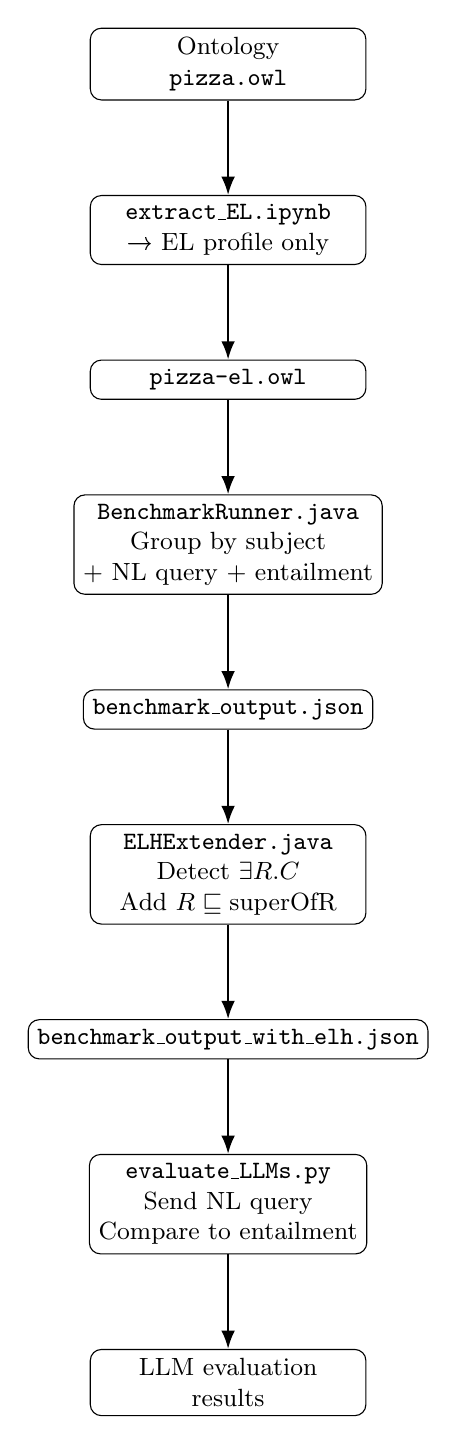
\begin{tikzpicture}[
        node distance=1.2cm and 2.5cm,
        every node/.style={draw, rounded corners, align=center, font=\small, minimum width=3.5cm},
        arrow/.style={-{Latex}, thick}
    ]

    \node (ont) {Ontology\\\texttt{pizza.owl}};
    \node (el) [below=of ont] {\texttt{extract\_EL.ipynb}\\→ EL profile only};
    \node (elowl) [below=of el] {\texttt{pizza-el.owl}};
    \node (bench) [below=of elowl] {\texttt{BenchmarkRunner.java}\\Group by subject\\+ NL query + entailment};
    \node (benchout) [below=of bench] {\texttt{benchmark\_output.json}};
    \node (elh) [below=of benchout] {\texttt{ELHExtender.java}\\Detect $\exists R.C$\\Add $R \sqsubseteq \text{superOfR}$};
    \node (elhout) [below=of elh] {\texttt{benchmark\_output\_with\_elh.json}};
    \node (eval) [below=of elhout] {\texttt{evaluate\_LLMs.py}\\Send NL query\\Compare to entailment};
    \node (res) [below=of eval] {LLM evaluation\\results};

    \draw [arrow] (ont) -- (el);
    \draw [arrow] (el) -- (elowl);
    \draw [arrow] (elowl) -- (bench);
    \draw [arrow] (bench) -- (benchout);
    \draw [arrow] (benchout) -- (elh);
    \draw [arrow] (elh) -- (elhout);
    \draw [arrow] (elhout) -- (eval);
    \draw [arrow] (eval) -- (res);

    \end{tikzpicture}
    \caption{Overview of the DL Reasoning Benchmarking Framework Pipeline}
    \label{fig:pipeline} 
\end{figure}

\newpage

The pipeline consists of four stages:

\begin{enumerate}
    \item \textbf{EL Ontology Extraction:} A subset of axioms conforming to the EL profile is extracted from the Pizza ontology using \texttt{extract\_EL.ipynb}. The output is an EL-compliant OWL file.
    
    \item \textbf{Benchmark Generation:} Java programs parse the EL ontology to group axioms by subject (\texttt{AxiomGrouper.java}), generate corresponding natural language queries (\texttt{QueryGenerator.java}), and compute ground-truth entailment using the HermiT reasoner (\texttt{ReasoningValidator.java}). **For validation, we primarily used the HermiT reasoner. Initial testing also involved validating axioms using the OWL API's structural reasoner, which yielded identical results for these simpler axiom groups. This consistency suggests that for the current level of complexity, both reasoners agree; however, for future investigations involving more complex scenarios and multiple metamorphic relation types, we plan to re-evaluate and compare their outputs more thoroughly.** These are saved in \texttt{benchmark\_output.json}.
    
    \item \textbf{ELH Extension:} The benchmark is enriched with role inclusion axioms to form ELH cases using \texttt{ELHExtender.java}, resulting in \texttt{benchmark\_output\_with\_elh.json}.
    
    \item \textbf{LLM Evaluation:} A Python script sends natural language queries to various LLMs (GPT-4o, Gemini, Gemma, LLaMA, etc.) using their APIs and compares their Yes/No predictions to ground-truth entailment.
\end{enumerate}

\subsection{DL Profiles and Scope}
The benchmark supports:
\begin{itemize}
    \item \textbf{EL:} A subset of DL supporting intersection and existential quantification
    \item \textbf{ELH:} EL extended with role hierarchy axioms (e.g., $r \sqsubseteq s$)
\end{itemize}
At this stage, no additional MR (metamorphic relation) types have been applied beyond the original EL/ELH logical transformations.

\subsection{Evaluation Metrics}
Model performance is measured by:
\begin{itemize}
    \item \textbf{Accuracy:} Match between model prediction and ground-truth entailment
    \item \textbf{False Positives / Negatives:} Detailed failure mode analysis
    \item \textbf{Execution Time:} Time required to evaluate all queries
    \item \textbf{Stability:} Detection of model errors, API failures, or hallucinated content
\end{itemize}


\section{Results and Analysis}

We evaluated seven large language models (LLMs) on a benchmark dataset derived from the Pizza ontology, focusing on two Description Logic fragments: EL and ELH. The benchmark measures entailment performance across simple subclass axioms and more complex role inclusion axioms. We report both raw accuracy and qualitative behavior per model.

\subsection{Entailment Accuracy}
\begin{table}[H]
\centering
\caption{Entailment Accuracy on EL and ELH}
\label{tab:accuracy}
\begin{tabular}{|l|c|c|c|}
\hline
\textbf{Model} & \textbf{EL Accuracy} & \textbf{ELH Accuracy} & \textbf{Total Accuracy} \\
\hline
GPT-4o* & \textbf{100.0 (58/58)\%} & \textbf{100.0 (58/58)\%} & \textbf{100.0\%} \\
Gemma 2 (4.3B Instruct) & \textbf{100.0 (58/58)\%} & 98.28 (57/58)\% & 99.14\% \\
Gemini 2.5 Pro & 98.28 (57/58)\% & 98.28 (57/58)\% & 98.28\% \\
Mistral (7B Instruct) & 94.83 (55/58)\% & 94.83 (55/58)\% & 94.83\% \\
Qwen 7B & 39.66 (23/58)\% & 32.76 (19/58)\% & 36.21\% \\
LLaMA 3 (8B Instruct) & 86.21 (50/58)\% & 81.03 (47/58)\% & 83.62\% \\
DeepSeek Coder (6.7B Instruct)* & 20.69 (12/58)\% & 15.52 (9/58)\% & 18.11\% \\
\hline
\end{tabular}
\end{table}

\subsection{Model Behavior Summary}
\begin{table}[H]
\scriptsize
\centering
\caption{Model Behavior Comparison Summary}
\label{tab:behavior}
\begin{tabular}{|l|c|c|c|c|c|c|c|}
\hline
\textbf{Feature} & \textbf{GPT-4o} & \textbf{Gemini} & \textbf{LLaMA 3} & \textbf{Gemma 3} & \textbf{Mistral} & \textbf{Qwen 7B} & \textbf{DeepSeek} \\
\hline
EL accuracy (\%) & 100.0 & 98.28 & 86.21 & 100.0 & 94.83 & 39.66 & 20.69 \\
ELH accuracy (\%) & 100.0 & 98.28 & 81.03 & 98.28 & 94.83 & 32.76 & 15.52 \\
Accuracy drop (\%) & 0.00 & 0.00 & 5.18 & 1.72 & 0.00 & 6.90 & 5.17 \\
False positives (count) & 0 & 0 & 0 & 0 & 0 & 0 & 0 \\
False negatives (count) & 0 & 1 & 8–11 & 1 & 3 & 35+ & 46–49 \\
Execution time & ~45s & ~10+ mins & ~30s & ~22s & ~35s & ~30s & ~4.5 mins \\
500 error occurrence & 0 & 2 & 0 & 0 & 0 & 0 & 0 \\
\hline
\end{tabular}
\end{table}


\subsection{Structural vs. HermiT Reasoner Runtime Comparison}

To validate entailment ground-truths, we used both the OWL API's \textbf{StructuralReasoner} and the \textbf{HermiT} reasoner. While both yielded consistent results for all EL test cases (i.e., the same entailment decisions), their runtime behavior differed substantially.

\begin{table}[h!]
\centering
\caption{Average Runtime per Entailment Check (in nanoseconds)}
\label{tab:reasoner-runtime}
\begin{tabular}{|l|c|c|}
\hline
\textbf{Reasoner} & \textbf{Min Time (ns)} & \textbf{Max Time (ns)} \\
\hline
StructuralReasoner & 5,584 & 84,733 \\
HermiT Reasoner & 118,958 & 659,709 \\
\hline
\end{tabular}
\end{table}

The \textbf{StructuralReasoner}, which uses syntactic approximation and supports tractable fragments like EL, consistently achieved inference times under 20 microseconds. In contrast, \textbf{HermiT}, a complete tableau-based reasoner, required up to 660 microseconds due to its support for more expressive DLs and complete reasoning.

Despite the significant runtime gap, both reasoners agreed on all entailments in the EL test set. This agreement stems from the simplicity of the benchmark cases, which strictly conform to the OWL~2 EL profile—a fragment designed for efficient reasoning and fully supported by both systems.

This validates the use of StructuralReasoner for efficient EL benchmarking while justifying HermiT’s role in future evaluations involving more complex logics (e.g., ELH, ALC) or structural transformations under metamorphic testing.

\subsection{Analysis}

Gemma 3 outperformed all other models in both EL and ELH benchmarks, achieving near-perfect accuracy with only a single false negative under ELH. Its strong performance suggests robust internal modeling of both subclass and role hierarchy semantics.

GPT-4o also performed well but showed a noticeable 5\% drop in ELH, indicating some sensitivity to the increased complexity introduced by role inclusions. Gemini 2.5 Pro was highly accurate and consistent across both EL and ELH but had one subtle semantic miss that prevented a perfect score.

Mistral demonstrated strong and reliable performance, particularly in subclass chains and ABox entailment. LLaMA 3 consistently underperformed, producing a high number of false negatives that suggest weaker internal logical structure. Qwen could resolve simple surface-level entailments but failed under existential quantifiers and complex role hierarchies.

DeepSeek Coder was unable to generalize to DL-based inputs and achieved only 1.72\% accuracy, making it unsuitable for reasoning tasks involving symbolic knowledge.

\subsection{Runtime and Stability}

Gemma and GPT-4o offered a strong tradeoff between accuracy and inference time. Gemini had the longest average runtime due to API latency but remained one of the most accurate. Notably, Gemini also faced occasional server instability (500 errors) that other models did not encounter.

All other models showed consistent runtime and stable API behavior.

\section{Conclusion and Future Work}
This study presents a comprehensive framework for benchmarking the reasoning capabilities of large language models (LLMs) using Description Logic (DL), specifically focusing on the EL and ELH fragments. By translating logical axioms into natural language queries and comparing model predictions against formal entailment results, we revealed substantial differences in model behavior, logical generalization, and sensitivity to DL complexity.

Our findings show that models like \textbf{Gemma 3} and \textbf{Mistral} demonstrate high reliability in DL-style tasks, including subclass chaining and role inclusion. In contrast, \textbf{LLaMA 3} and \textbf{DeepSeek Coder} exhibit significant deficiencies, particularly under ELH settings. \textbf{Gemini 2.5 Pro} and \textbf{GPT-4o} perform well overall, though GPT-4o shows minor degradation when handling extended logical structures.

Future work includes:
\begin{itemize}
    \item Implementing and evaluating more metamorphic reasoning types (e.g., paraphrasing, axiom removal)
    \item Expanding to additional DL fragments such as ALC or SHOIN
    \item Applying fine-tuning or prompt engineering to guide model reasoning more effectively
    \item Incorporating formal proof explanations alongside binary entailment responses
\end{itemize}

\newpage

\bibliographystyle{plain}
\bibliography{references}
\nocite{*}

\end{document}
